\chapter{Using Skel}

\section{Requirements}
Skel is bundled with ADIOS, and thus requires a system capable of building ADIOS on. In addition there are a couple of extra python packages that may be required to use all of the features of skel. 

Skel has been tested to work with Python 2.7. Other versions of python may or may not work.

You will need Cheetah, which is free and open source software. Instructions for installing
Cheetah may be found here: www.cheetahtemplate.org/docs/users\_guide\_html/users\_guide.html
This version of Skel has been tested with version 2.4.4 of Cheetah.

You will also need the PyYAML package. Instructions for downloading and installing 
PyYAML may be found here: http://pyyaml.org/wiki/PyYAML. This version of Skel has been
tested with version 3.10 of PyYaml.

On Linux systems, you may be able to find these packages in your package manager's library,
which may simplify the installation process. 


\section{Overview of Manual Benchmark Creation}
Figure \ref{fig:overview}  shows the typical workflow of using skel to create a skeletal I/O 
benchmark. The example uses the GTS application, and thus the workflow begins
with gts.xml, the XML descriptor from GTS. The {\it skel xml} command is used
to create a second xml file, gts\_skel.xml which will serve as the ADIOS xml
descriptor for the skeletal application. Next, skel params is used to generate
a parameters file. The generated parameters file is then edited by the user to
guide the subsequent generation of the skeletal application.

\begin{figure}[htb]
  \center{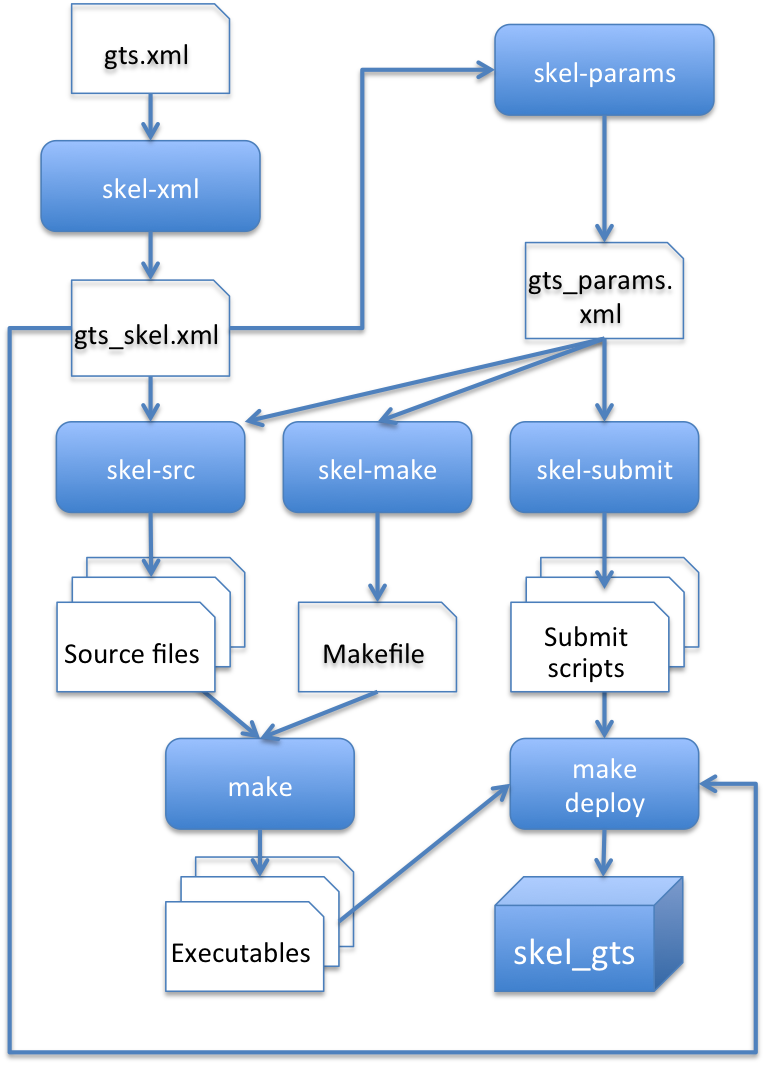
\includegraphics[width=75mm]
  {figures/overview.png}}
  \caption{\label{fig:overview} Skel Workflow}
\end{figure}

%Figure 1: Skel Workflow

At this point, the commands {\it skel source}, {\it skel makefile}, and {\it skel submit}
may be used to generate the source files, Makefile, and submission scripts that
comprise the skeletal application. With all of the components of the skeletal
application created, it is now time to build the application, using {\it make}, and
finally deploy the application to a directory from which it may be launched,
using {\it make deploy}, which copies the gts\_skel.xml file, executable files, and
submission script. The user now has a ready to run I/O benchmark without
having written any source code at all.



\section{Detailed Example of Manual Benchmark Creation}
In this section we will describe the steps used to create an I/O Kernel based
on the GTS application. The ADIOS config file for GTS can be found in the
examples directory.

The steps are

{\tt skel xml gts}

{\tt skel params gts}

Edit the parameters file, particularly the values of scalars that control array sizes,
and the desired tests to run.

{\tt skel makefile gts}

{\tt skel source gts}

{\tt skel submit gts} (optional)

{\tt make}

{\tt make deploy} (optional)



\section{Recreating a Run Using Skel Replay (Experimental)}
We have added a feature in this release that allows a benchmark to be created
automatically based on an existing bp file. This replay feature eliminates the
tedious nature of creating and tweaking a parameter file, instead taking that 
information directly from the bp file, settings file, or command line, in order
to allow direct replay while simplifying the steps that a user must take.

To show the usage of the replay feature, assume we have a bp file, out.bp,
that was produced by an application called myapp. Generating a benchmark based on out.bp is simple: 

{\tt skel replay myapp -b out.bp}

This single command generates an adios XML file, source code, a makefile, and a submission script, and finally executes the makefile, providing a ready to run benchmark.

\section{Using Skel for a remote replay (Experimental)}

In the case where you have a large bp file representing an I/O pattern you want to run
on a different machine, it may be desirable to extract the metadata information from the
bp file, rather than transferring the entire file to the remote machine. To
accomplish this, simply use the skeldump command as follows:

{\tt skeldump out.bp > out.yaml}

Skeldump creates a yaml file containing all of the information required to build the
benchmark on the remote machine. After moving only the yaml file to the remote machine,
the benchmark creation can be accomplished with:

{\tt skel replay myapp -y out.yaml}

